\documentclass[12pt,a4paper]{article}
\usepackage[margin=2cm]{geometry}
\usepackage{xeCJK}
\usepackage{fontspec}
\setCJKmainfont{Noto Serif CJK TC}[Script=CJK]
\usepackage{amsmath,amssymb}
\usepackage{graphicx}
\usepackage{fancyhdr}
\setlength{\headheight}{14.5pt}
\addtolength{\topmargin}{-2.5pt}
\usepackage{hyperref}
\usepackage{listings}
\usepackage{enumitem}
\usepackage{titlesec}
\usepackage{caption}
\usepackage{indentfirst}
\usepackage{booktabs}
\usepackage{longtable}
\usepackage{multirow}
\usepackage{array}
\usepackage{tabularx}
\usepackage{float}
\usepackage{minted}
\usepackage{tikz}
\usetikzlibrary{positioning,arrows.meta}

\setlength{\parindent}{2em}
\pagestyle{fancy}
\fancyhf{}
\cfoot{\thepage}
\linespread{1.3}
\setminted{
    linenos,                % 行號
    frame=lines,            % 上下框線
    framesep=5pt,           % 程式碼與邊框距離
    numbersep=8pt,          % 行號與程式碼距離
    fontsize=\scriptsize,   % 字體大小
    breaklines,             % 自動換行
    tabsize=4,              % tab 寬度
    rulecolor=\color{black},% 框線顏色
    xleftmargin=1.5em       % 左側縮排
}

\title{Fundamentals of Biomedical Image Processing HW 1}
\author{B12508026戴偉璿}
\date{\today}


\begin{document}

\maketitle
\lhead{Fundamentals of Biomedical Image Processing Homework 1}
\rhead{B12508026戴偉璿}

\section{Theorem questions}
\begin{enumerate}
    \item
    \begin{enumerate}
        \item The picture size is $1024\times 1024$ pixels, and each pixel contains 256 intensity levels(8 bits,i.e., 1 byte). Therefore, the total data size is $1024\times 1024 \times 1 = 1,048,576$ bytes. Since each packet requires 10 bits to transmit 1 byte of data, the total number of bits to be transmitted is 10,485,760 bits. With the baud rate of 56k, the transmission time is $10,485,760\div 56000 \approx 187.25(sec)\approx 3.12$ minutes.
        \item With the baud rate of 3000k, the transmission time is\\ $10,485,760\div 3,000,000 \approx 3.495(sec)\approx 0.058$ minutes.
    \end{enumerate}
    \item $V=\{1 ,2\}$, so the graph would be Fig \ref{fig:2a}:
    \begin{figure}[H]
        \centering
        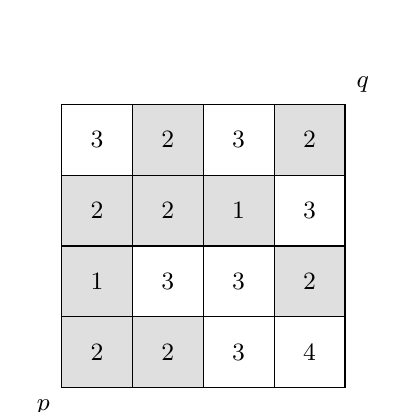
\begin{tikzpicture}[scale=0.9, every node/.style={font=\small}][H]
  %----- 基本參數 -----
  \def\cell#1#2#3{ % (row, col, value)
    % 座標:左下(1,1),右上(4,4);但我們用 top-down 排列所以要轉換
    \pgfmathsetmacro{\x}{#2-1}
    \pgfmathsetmacro{\y}{4-#1}
    % 填色:V={1,2} 可走(light gray),其他白色
    \ifnum#3<3
      \fill[gray!25] (\x,\y) rectangle ++(1,1);
    \else
      \fill[white]   (\x,\y) rectangle ++(1,1);
    \fi
    % 外框
    \draw (\x,\y) rectangle ++(1,1);
    % 數字
    \node at (\x+0.5,\y+0.5) {\small #3};
  }
  %----- 填資料(row, col, value) -----
  % Row 1 (top): 3 2 3 2(q)
  \cell{1}{1}{3}  \cell{1}{2}{2}  \cell{1}{3}{3}  \cell{1}{4}{2}
  % Row 2: 2 2 1 3
  \cell{2}{1}{2}  \cell{2}{2}{2}  \cell{2}{3}{1}  \cell{2}{4}{3}
  % Row 3: 1 3 3 2
  \cell{3}{1}{1}  \cell{3}{2}{3}  \cell{3}{3}{3}  \cell{3}{4}{2}
  % Row 4 (bottom): 2(p) 2 3 4
  \cell{4}{1}{2}  \cell{4}{2}{2}  \cell{4}{3}{3}  \cell{4}{4}{4}

  %----- 標記 p 與 q -----
  % p at (row=4,col=1) -> (x=0,y=0)
  \node[below left=1pt] at (0,0) {$p$};
  % q at (row=1,col=4) -> (x=3,y=3)
  \node[above right=1pt] at (4,4) {$q$};

%   %----- shortest-8(藍色,長度 4): p(4,1)->(3,1)->(2,2)->(2,3)->q(1,4) -----
%   \draw[very thick,blue,-{Stealth[length=3mm]}]
%     (0.5,0.5) -- (0.5,1.5) -- (1.5,2.5) -- (2.5,2.5) -- (3.5,3.5);

%   %----- shortest-m(橙色,長度 5): p->(3,1)->(2,1)->(2,2)->(2,3)->q -----
%   \draw[very thick,orange!90!black,-{Stealth[length=3mm]}]
%     (0.5,0.5) -- (0.5,1.5) -- (0.5,2.5) -- (1.5,2.5) -- (2.5,2.5) -- (3.5,3.5);

%   %----- 圖例 -----
%   \draw[very thick,blue]   (0.1,-0.7)--+(0.6,0) node[right,black]{shortest-8 length $=4$};
%   \draw[very thick,orange!90!black] (2.6,-0.7)--+(0.6,0) node[right,black]{shortest-m length $=5$};
%   \node[black] at (2,-1.2) {shortest-4: no 4-connected path (q is 4-blocked)};
\end{tikzpicture}
        \caption{The grid graph with $V=\{1,2\}$ (gray cells are passable)}
        \label{fig:2a}
    \end{figure}
    \newpage
    \begin{enumerate}
        \item \fbox{shortest-4}: Only up, down, left, right movements are allowed. So the path would be:
        \begin{figure}[H]
            \centering
            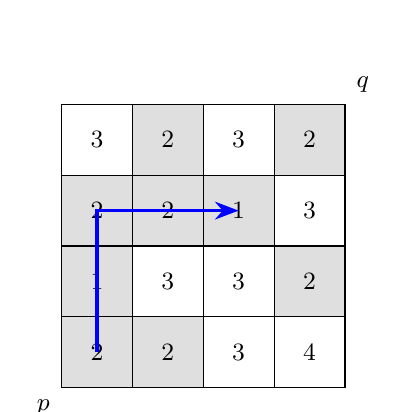
\begin{tikzpicture}[scale=0.9, every node/.style={font=\small}][H]
  %----- 基本參數 -----
  \def\cell#1#2#3{ % (row, col, value)
    % 座標:左下(1,1),右上(4,4);但我們用 top-down 排列所以要轉換
    \pgfmathsetmacro{\x}{#2-1}
    \pgfmathsetmacro{\y}{4-#1}
    % 填色:V={1,2} 可走(light gray),其他白色
    \ifnum#3<3
      \fill[gray!25] (\x,\y) rectangle ++(1,1);
    \else
      \fill[white]   (\x,\y) rectangle ++(1,1);
    \fi
    % 外框
    \draw (\x,\y) rectangle ++(1,1);
    % 數字
    \node at (\x+0.5,\y+0.5) {\small #3};
  }
  %----- 填資料(row, col, value) -----
  % Row 1 (top): 3 2 3 2(q)
  \cell{1}{1}{3}  \cell{1}{2}{2}  \cell{1}{3}{3}  \cell{1}{4}{2}
  % Row 2: 2 2 1 3
  \cell{2}{1}{2}  \cell{2}{2}{2}  \cell{2}{3}{1}  \cell{2}{4}{3}
  % Row 3: 1 3 3 2
  \cell{3}{1}{1}  \cell{3}{2}{3}  \cell{3}{3}{3}  \cell{3}{4}{2}
  % Row 4 (bottom): 2(p) 2 3 4
  \cell{4}{1}{2}  \cell{4}{2}{2}  \cell{4}{3}{3}  \cell{4}{4}{4}

  %----- 標記 p 與 q -----
  % p at (row=4,col=1) -> (x=0,y=0)
  \node[below left=1pt] at (0,0) {$p$};
  % q at (row=1,col=4) -> (x=3,y=3)
  \node[above right=1pt] at (4,4) {$q$};

  %----- shortest-8(藍色,長度 4): p(4,1)->(3,1)->(2,2)->(2,3)->q(1,4) -----
  \draw[very thick,blue,-{Stealth[length=3mm]}]
    (0.5,0.5) -- (0.5,1.5) -- (0.5,2.5) -- (1.5,2.5) -- (2.5,2.5) ;

%   %----- shortest-m(橙色,長度 5): p->(3,1)->(2,1)->(2,2)->(2,3)->q -----
%   \draw[very thick,orange!90!black,-{Stealth[length=3mm]}]
%     (0.5,0.5) -- (0.5,1.5) -- (0.5,2.5) -- (1.5,2.5) -- (2.5,2.5) -- (3.5,3.5);

%   %----- 圖例 -----
%   \draw[very thick,blue]   (0.1,-0.7)--+(0.6,0) node[right,black]{shortest-8 length $=4$};
%   \draw[very thick,orange!90!black] (2.6,-0.7)--+(0.6,0) node[right,black]{shortest-m length $=5$};
%   \node[black] at (2,-1.2) {shortest-4: no 4-connected path (q is 4-blocked)};
\end{tikzpicture}
            \caption{No 4-connected path (q is 4-blocked)}
            \label{fig:2a_s4}
        \end{figure}
        As the Fig\ref{fig:2a_s4} shows, there's no path from last step $(3, 3)$ to node $q(4, 4)$, so the length is \textbf{infinity}.
        \item \fbox{shortest-8}: Up, down, left, right, and diagonal movements are allowed. So the path would be:
        \begin{figure}[H]
            \centering
            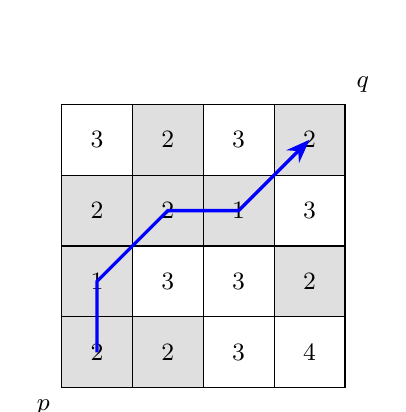
\begin{tikzpicture}[scale=0.9, every node/.style={font=\small}][H]
  %----- 基本參數 -----
  \def\cell#1#2#3{ % (row, col, value)
    % 座標:左下(1,1),右上(4,4);但我們用 top-down 排列所以要轉換
    \pgfmathsetmacro{\x}{#2-1}
    \pgfmathsetmacro{\y}{4-#1}
    % 填色:V={1,2} 可走(light gray),其他白色
    \ifnum#3<3
      \fill[gray!25] (\x,\y) rectangle ++(1,1);
    \else
      \fill[white]   (\x,\y) rectangle ++(1,1);
    \fi
    % 外框
    \draw (\x,\y) rectangle ++(1,1);
    % 數字
    \node at (\x+0.5,\y+0.5) {\small #3};
  }
  %----- 填資料(row, col, value) -----
  % Row 1 (top): 3 2 3 2(q)
  \cell{1}{1}{3}  \cell{1}{2}{2}  \cell{1}{3}{3}  \cell{1}{4}{2}
  % Row 2: 2 2 1 3
  \cell{2}{1}{2}  \cell{2}{2}{2}  \cell{2}{3}{1}  \cell{2}{4}{3}
  % Row 3: 1 3 3 2
  \cell{3}{1}{1}  \cell{3}{2}{3}  \cell{3}{3}{3}  \cell{3}{4}{2}
  % Row 4 (bottom): 2(p) 2 3 4
  \cell{4}{1}{2}  \cell{4}{2}{2}  \cell{4}{3}{3}  \cell{4}{4}{4}

  %----- 標記 p 與 q -----
  % p at (row=4,col=1) -> (x=0,y=0)
  \node[below left=1pt] at (0,0) {$p$};
  % q at (row=1,col=4) -> (x=3,y=3)
  \node[above right=1pt] at (4,4) {$q$};

  %----- shortest-8(藍色,長度 4): p(4,1)->(3,1)->(2,2)->(2,3)->q(1,4) -----
  \draw[very thick,blue,-{Stealth[length=3mm]}]
    (0.5,0.5) -- (0.5,1.5) -- (1.5,2.5) -- (2.5,2.5) -- (3.5,3.5);

%   %----- shortest-m(橙色,長度 5): p->(3,1)->(2,1)->(2,2)->(2,3)->q -----
%   \draw[very thick,orange!90!black,-{Stealth[length=3mm]}]
%     (0.5,0.5) -- (0.5,1.5) -- (0.5,2.5) -- (1.5,2.5) -- (2.5,2.5) -- (3.5,3.5);

%   %----- 圖例 -----
%   \draw[very thick,blue]   (0.1,-0.7)--+(0.6,0) node[right,black]{shortest-8 length $=4$};
%   \draw[very thick,orange!90!black] (2.6,-0.7)--+(0.6,0) node[right,black]{shortest-m length $=5$};
%   \node[black] at (2,-1.2) {shortest-4: no 4-connected path (q is 4-blocked)};
\end{tikzpicture}
            \caption{shortest-8 path (length = 4)}
            \label{fig:2a_s8}
        \end{figure}
        As the Fig\ref{fig:2a_s8} shows, it takes 4 steps to reach from $p(1, 1)$ to $q(4, 4)$,\\ so the length is \textbf{4}.
        \newpage
        \item \fbox{shortest-m}: The path can only move to the 8-neighbors with the minimum value. So the path would be:
        \begin{figure}[H]
            \centering
            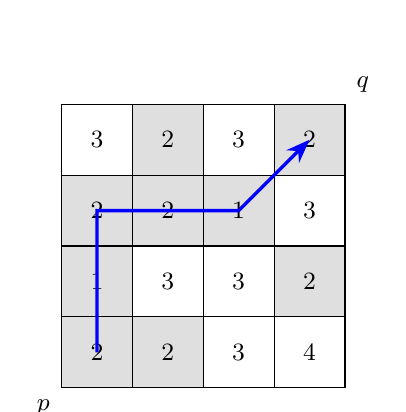
\begin{tikzpicture}[scale=0.9, every node/.style={font=\small}][H]
  %----- 基本參數 -----
  \def\cell#1#2#3{ % (row, col, value)
    % 座標:左下(1,1),右上(4,4);但我們用 top-down 排列所以要轉換
    \pgfmathsetmacro{\x}{#2-1}
    \pgfmathsetmacro{\y}{4-#1}
    % 填色:V={1,2} 可走(light gray),其他白色
    \ifnum#3<3
      \fill[gray!25] (\x,\y) rectangle ++(1,1);
    \else
      \fill[white]   (\x,\y) rectangle ++(1,1);
    \fi
    % 外框
    \draw (\x,\y) rectangle ++(1,1);
    % 數字
    \node at (\x+0.5,\y+0.5) {\small #3};
  }
  %----- 填資料(row, col, value) -----
  % Row 1 (top): 3 2 3 2(q)
  \cell{1}{1}{3}  \cell{1}{2}{2}  \cell{1}{3}{3}  \cell{1}{4}{2}
  % Row 2: 2 2 1 3
  \cell{2}{1}{2}  \cell{2}{2}{2}  \cell{2}{3}{1}  \cell{2}{4}{3}
  % Row 3: 1 3 3 2
  \cell{3}{1}{1}  \cell{3}{2}{3}  \cell{3}{3}{3}  \cell{3}{4}{2}
  % Row 4 (bottom): 2(p) 2 3 4
  \cell{4}{1}{2}  \cell{4}{2}{2}  \cell{4}{3}{3}  \cell{4}{4}{4}

  %----- 標記 p 與 q -----
  % p at (row=4,col=1) -> (x=0,y=0)
  \node[below left=1pt] at (0,0) {$p$};
  % q at (row=1,col=4) -> (x=3,y=3)
  \node[above right=1pt] at (4,4) {$q$};

  %----- shortest-8(藍色,長度 4): p(4,1)->(3,1)->(2,2)->(2,3)->q(1,4) -----
  \draw[very thick,blue,-{Stealth[length=3mm]}]
    (0.5,0.5) -- (0.5,1.5) -- (0.5,2.5) -- (1.5,2.5) -- (2.5,2.5) -- (3.5,3.5);

%   %----- shortest-m(橙色,長度 5): p->(3,1)->(2,1)->(2,2)->(2,3)->q -----
%   \draw[very thick,orange!90!black,-{Stealth[length=3mm]}]
%     (0.5,0.5) -- (0.5,1.5) -- (0.5,2.5) -- (1.5,2.5) -- (2.5,2.5) -- (3.5,3.5);

%   %----- 圖例 -----
%   \draw[very thick,blue]   (0.1,-0.7)--+(0.6,0) node[right,black]{shortest-8 length $=4$};
%   \draw[very thick,orange!90!black] (2.6,-0.7)--+(0.6,0) node[right,black]{shortest-m length $=5$};
%   \node[black] at (2,-1.2) {shortest-4: no 4-connected path (q is 4-blocked)};
\end{tikzpicture}
            \caption{shortest-m path (length = 5)}
            \label{fig:2a_sm}
        \end{figure}
        As the Fig\ref{fig:2a_sm} shows, it takes 5 steps to reach from $p(1, 1)$ to $q(4, 4)$,\\ so the length is \textbf{5}.
    \end{enumerate}
\end{enumerate}

\section{Programming exercises}

All code is stored at the 


\begin{enumerate}
    \item 
\end{enumerate}


\end{document}